\subsection{Truncated Cone}

\begin{figure}[H]
  \centering 
  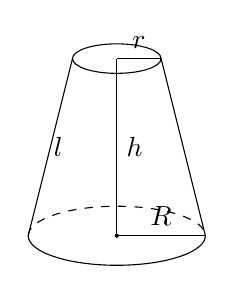
\begin{tikzpicture}[scale=0.75] % Draw top ellipse 
      \draw (0,0) ellipse (0.75 and 0.25);

      % Draw bottom ellipse
      \draw (-1.5,-3.0) arc (180:360:1.5 and 0.5);
      \draw [dashed] (-1.5,-3.0) arc (180:360:1.5 and -0.5);

      % Draw side lines
      \draw (-0.75,0) -- (-1.5,-3.0);
      \draw (1.5,-3.0) -- (0.75,0);  

      % Draw height line
      \draw (0, -3.0) -- node[midway, right] { $h$ } (0,0);  

      % Draw radii lines
      \draw (0, -3.0) -- node[midway, above] { $R$ } (1.5, -3.0);
      \draw (0, 0.0) -- node[midway, above] { $r$ } (0.75, 0.0);


      % Add labels
      \node at (-0.75, -1.5) [left] { $l$ };

      % Mark center point
      \fill (0, -3.0) circle [radius=1pt];
  \end{tikzpicture}
\end{figure}

\subsubsection{Area}

\[
  l = \sqrt(h^2 + l^2) 
\]

\[
  A  = \pi (R+r) l + \pi (R^2 + r^2)
\]

\subsubsection{Volume}

\[
    V = \frac{1}{3}\pi h(R^2 + Rr + r^2),
\]

